\documentclass[12pt,a4paper,titlepage]{article}
%va sempre messo article per "program documentation"
\usepackage[italian]{babel}
\usepackage[T1]{fontenc}
\usepackage[latin1]{inputenc}
\usepackage{titlesec}
\usepackage[hidelinks]{hyperref}
\usepackage[a4paper,top=2cm,bottom=2cm,left=1cm,right=1cm]{geometry}
\usepackage{soulutf8,color}
\usepackage{multirow}
\usepackage{lscape}
\usepackage{graphicx}
\usepackage{eurosym} %per il simbolo dell' \euro


\usepackage{emptypage} 
% pagine vuote senza testatina e piede di pagina

%\usepackage{hyperref} 
% collegamenti ipertestuali

\usepackage{fancyhdr}
% pacchetto per intestazione e pie pagina

\pagestyle{fancy}


% \\ indica interruzione di riga

% compilate 2 volte per documenti con indice

% {\em qui testo in corsivo}
% {\bfseries qui testo in grossetto}

%LISTE NUMERATE
%\begin{enumerate}
%\item primo
%\item secondo
%\item terzo
%\end{enumerate}

%LISTE PUNTATE
%\begin{itemize}
%\item primo
%\item secondo
%\item \dots
%\end{itemize}

%TABELLA
%\begin{tabular}{|c|c|c|}
%indica una tabella con 3 colonne e pos. testo centrale. La barra verticale ( | ) indica che vi è una linea divisoria verticale tra le celle.
%\hline	linea separatrice orizzontale
%testo1& testo2& testo3\\
% & segna la fine del testo nella cella, \\ indica il fine della riga 

\newcommand{\minitab}[2][1]{\begin{tabular}#1 #2\end{tabular}}

%GRAFICI
%\begin{figure}
%\includegraphics{filegrafico}
%comando per includere le immagini (controllare i formati)
%\caption{didascalia}
%\label{nome}
%\end{figure}

%----------------------------------------------------------- INIZIO TEMPLATE TITOLO

\usepackage{xcolor} % Importa i colori per la prima pagina
\usepackage{fix-cm} % Permette l'incremento del font oltre misura

\newcommand{\HRule}[1]{\hfill \rule{0.2\linewidth}{#1}} % Horizontal rule at the bottom of the page, adjust width here

\definecolor{grey}{rgb}{0.9,0.9,0.9} % Colore del box del titolo

\begin{document}
	
	\thispagestyle{empty} % Toglie il numero della pagina nella prima pagina
	
	%----------------------------------------------------------------------------------------
	%	TITLE SECTION
	%----------------------------------------------------------------------------------------
	
	\colorbox{grey}{
		\parbox[t]{1.0\linewidth}{
			\centering \fontsize{50pt}{80pt}\selectfont % Il primo è la grandezza del font, il secondo lo spazio lasciato
			\vspace*{0.7cm} % Spazio dall'inizio del box al titolo
			
			\raggedleft
			
\includegraphics[width=0.7\linewidth]{../../LogoSWEgGroupSFONDOVUOTO}
			
			\hfill Piano di Progetto \\
			
			\vspace*{0.7cm} % Spazio dalla fine del testo alla fine del box
		}
	}
	
	%----------------------------------------------------------------------------------------
	
	\vfill % Spazio dalla fine del box alle altre informazioni
	
	%----------------------------------------------------------------------------------------
	%	Informazioni sul documento
	%----------------------------------------------------------------------------------------
	
	{\centering \large 
		\hfill \textbf{Versione} 1.0.0 \\
		\hfill \textbf{Redazione} Sebastiano Marchesini \\
		\hfill Piergiorgio Danieli \\
		\hfill \textbf{Verifica} Pietro Lonardi \\
		\hfill \textbf{Validazione} Alberto Gelmi \\
		\hfill \textbf{Responsabile} Sebastiano Marchesini \\
		\hfill \textbf{Uso} Interno \\
		\hfill \textbf{Destinato} SWEg Group \\ 
		
		\HRule{1pt}
		
		\textbf{Sommario} \\
	    Questo documento ha l'obiettivo di misurare l'efficienza e pianificare i processi del progetto.
		
	} % Linea orizzontale di estetica
	
	
	%----------------------------------------------------------------------------------------
	
	\clearpage % Parta bianca finale della pagina
	
	%----------------------------------------------------------- FINE TEMPLATE TITOLO

\lhead{
\includegraphics[width=0.2\linewidth]{../../LogoSWEgGroup}}
\chead{}
\lfoot{Piano Di Progetto}
\cfoot{}
\rfoot{\thepage}
\renewcommand{\headrulewidth}{0.2pt}
\renewcommand{\footrulewidth}{0.2pt}

\rhead{Registro Modifiche}
\section{Registro Modifiche}
\small %rippicciolisce il testo

{\renewcommand\arraystretch{1.2} %aumenta l'altezza di ogni riga
\begin{tabular}{|l|c|c|c|}
		\hline
		{\textbf{Modifica}}&{\textbf{Nome}}&{\textbf{Data}}&{\textbf{Ver.}}\\
			\hline
			Validazione & Alberto Gelmi & 10/01/2017 & 1.0.0 \\
			\hline
			Correzioni Verifica & Sebastiano Marchesini & 09/01/2017 & 0.5.1 \\
			\hline
			Verifica & Pietro Lonardi & 09/01/2017 & 0.5.0 \\
			\hline
			Inserimento Tabelle & Sebastiano Marchesini & 05/01/2017 & 0.1.3 \\
			\hline
			Stesura finale & Sebastiano Marchesini & 04/01/2017 & 0.1.2 \\
			\hline
			Stesura modello sviluppo e preventivo & Piergiorgio Danieli & 03/01/2017 & 0.1.1 \\
			\hline
			Stesura primi capitoli documento & Sebastiano Marchesini & 02/01/2017 & 0.1.0 \\
			\hline
			Studio dei riferimenti e impostato il documento & Sebastiano Marchesini & 21/12/2016 & 0.0.1 \\
			\hline
\end{tabular}
}
\normalsize

\newpage

\tableofcontents
%crea indice automaticamente
\thispagestyle{empty}

\newpage


\rhead{Introduzione}
\section{Introduzione}
\subsection{Scopo del Documento}
Lo scopo generale del documento è di misurare l'efficienza e tenerla in considerazione preventivamente. Importantissimo per il committente che tiene d'occhio la stima delle risorse. \\
È in particolare una dichiarazione di interfaccia di pianificazione e consuntivazione. Sempre redatto dal \textit{Project Manager} schematizzato:
\begin{enumerate}
	\item Definizione degli obbiettivi;
	\item Analisi dei rischi;
	\item Descrizione del modello di processo di sviluppo;
	\item Suddivisione di sottoinsiemi;
	\item Attività di progetto;
	\item Stima dei costi;
	\item Consuntivo attività.
\end{enumerate} 

\subsection{Glossario}
Al fine di evitare ambiguità e ottimizzare la comprensione dei documenti, viene incluso un Glossario, nel quale saranno inseriti i termini tecnici, acronimi e parole che necessitano di essere chiarite.\\
Un glossario è una raccolta di termini di un ambito specifico e circoscritto. In questo caso per raccogliere termini desueti e specialistici inerenti al progetto. 

\subsection{Riferimenti}
\subsubsection{Normativi}
\begin{itemize}
	\item \textbf{Vincoli organigramma e dettagli tecnico-economici}: \\
	\textcolor{blue}{\url{http://www.math.unipd.it/~tullio/IS-1/2016/Progetto/PD01b.html}}.
	\item \textbf{Norme di Progetto}: \\
	"Norme di Progetto v1.0.0".
 \end{itemize}
\subsubsection{Informativi}
\begin{itemize}
	\item \textbf{Metriche di Progetto}: \\
	\textcolor{blue}{\url{https://it.wikipedia.org/wiki/Metriche_di_progetto}}.
	\item \textbf{Modello incrementale}: \\
	\textcolor{blue}{\url{https://it.wikipedia.org/wiki/Modello_incrementale}}.
	\item \textbf{Modello incrementale}: \\
	\textcolor{blue}{\url{https://it.wikipedia.org/wiki/Metodologia_agile}}.
	\item \textbf{Gestione di progetto}: \\
	\textcolor{blue}{\url{http://www.math.unipd.it/~tullio/IS-1/2016/Dispense/L04.pdf}}.
\end{itemize}

\newpage

\rhead{Scadenze}
\section{Scadenze}
\subsection{Scadenzario}
Tutte le date sono indicate per l'anno 2017.\\

{\renewcommand\arraystretch{1.2} %aumenta l'altezza di ogni riga
\begin{tabular}{|l|c|c|c|c|c|}
\hline
 & Consegna & \textbf{RR} & \textbf{RP} & \textbf{RQ} & \textbf{RA} \\
\hline
\textit{I°} & 11/01 & 24/01 & 13/03 & 18/04 & 15/05 \\
\textit{II°} & & 13/03 & 18/04 & 15/05 & 27/06 \\
\textit{III°} & & 18/04 & 15/05 & 27/06 & 13/07 \\
\textit{IV°} & & 15/05 & 27/06 & 13/07 & 29/08 \\
\textit{V°} & & 27/06 & 13/07 & 29/08 & 12/09 \\
\hline
\end{tabular}}
\vspace{0.5cm}
\\
E le sigle stanno a indicare rispettivamente:
\begin{enumerate}
	\item \textbf{RR}: Revisione dei Requisiti;
	\item \textbf{RP}: Revisione di Progettazione;
	\item \textbf{RQ}: Revisione di Qualifica;
	\item \textbf{RA}: Revisione di Accettazione. 
\end{enumerate}

Il gruppo si attiene a mantenere con efficienza le prime date di consegna per avere un prodotto finito nel mese di Maggio.

\subsection{Stati di avanzamento}
\subsubsection{Documentazione}
\small
{\renewcommand\arraystretch{1.2}
\begin{tabular}{|p{2cm}|p{5cm}|p{5cm}|}
	\hline
	\textbf{RR} & Analisi dei Requisiti & \begin{trivlist}
												\item Piano di Progetto v1
												\item Piano di Qualifica v1
												\item Norme di Progetto v1
													\end{trivlist}
												\\
	\textbf{RPmin} & Specifica Tecnica & \begin{trivlist}
			\item Piano di Progetto v2
			\item Piano di Qualifica v2
			\item Norme di Progetto v2
	\end{trivlist}
													\\
	\textbf{RPmax} & Definizione di Prodotto & \begin{trivlist}
		\item Piano di Progetto v3
		\item Piano di Qualifica v3
		\item Norme di Progetto v3
	\end{trivlist} \\
	\textbf{RQ} & Esito finale della Qualifica & \begin{trivlist}
		\item Piano di Progetto v4
		\item Piano di Qualifica v4
		\item Norme di Progetto v4
	\end{trivlist}\\
	\textbf{RA} & Collaudo di Accettazione & \begin{trivlist}
															\item Piano di Progetto v5
															\item Piano di Qualifica v5
											 \end{trivlist}\\ 
														 
\hline
\end{tabular}}

\normalsize
\subsection{Ciclo di revisioni}
\subsubsection{Revisione dei requisiti (RR)}
La Revisione dei requisiti è una delle uniche due revisioni bloccanti.\\
È importante concordare con il cliente una visione del prodotto atteso.\\
Prodotti interni valutati:
\begin{itemize}
	\item Studio di Fattibilità;
	\item Norme di Progetto v1;
\end{itemize}
Prodotti esterni valutati:
\begin{itemize}
	\item Analisi dei Requisiti;
	\item Piano di Qualifica v1;
	\item Piano di Progetto v1.
\end{itemize}

\subsubsection{Revisione di Progettazione}
Presenti due tipi di revisione di progettazione: MIN e MAX. \\
Rispettivamente uno accerta la realizzabilità l'altro accerta le caratteristiche del prodotto da realizzare\\
A partire da RPmin, cioè una progettazione di alto livello che presenta tra i prodotti interni:
\begin{itemize}
	\item Norme di Progetto v2;
\end{itemize}
Prodotti esterni valutati: 
\begin{itemize}
	\item Piano di Progetto v2;
	\item Piano di Qualifica v2;
	\item Specifica tecnica.
\end{itemize}
Segue la RPmax con una progettazione più a basso livello e l'aggiornamento dei prodotti interni:
\begin{itemize}
	\item Norme di Progetto v3;
\end{itemize}
ed esterni:
\begin{itemize}
	\item Piano di Progetto v3;
	\item Piano di Qualifica v3;
	\item Definizione del prodotto.
\end{itemize}

\subsubsection{Revisione di Qualifica}
La revisione di qualifica evidenzia che il prodotto sembri funzionare. \\
Revisione dell'esito finale di qualifiche delle verifiche e attivazione di validazione \\
Prodotti interni valutati:
\begin{itemize}
	\item Norme di Progetto v4;
\end{itemize}
Prodotti esterni valutati:
\begin{itemize}
	\item Piano di Qualifica v4;
	\item Piano di Progetto v4;
	\item Versione preliminare del Manuale Utente (MU v1);
\end{itemize}
Prodotti esterni forniti a scopo illustrativo:
\begin{itemize}
	\item DP finale.
\end{itemize}

\subsubsection{Revisione di Accettazione}
Collaudo di sistema per accettazione della parte committente.\\
Accertamento del soddisfacimento di tutti i requisiti utente pattuiti nella \textit{Revisione dei Requisiti}.\\
Prodotti esterni valutati:
\begin{itemize}
	\item Piano di Qualifica v5 con esito finale di verifica validazione;
	\item Piano di Progetto v5 consuntivo finale;
	\item Manuale Utente v2.
\end{itemize}

\newpage

\rhead{Analisi dei Rischi }
\section{Analisi dei Rischi}
Per un miglior avanzamento del progetto, si è effettuata un attenta analisi dei rischi. Per la loro gestione è stato scelto il seguente metodo: 
\begin{enumerate}
	\item \textbf{Identificazione}: trovare i vari rischi che possono trovarsi durante il processo e capirne il tipo. I rischi possono essere classificati in:
	\begin{itemize}
		\item \textit{Progetto}: relativi a pianificazione, strumenti ed alle risorse;
		\item \textit{Prodotto}: relativi a conformità alle aspettative del committente;
		\item \textit{Businnes}: relativi a costi e concorrenza.
	\end{itemize}
	\item \textbf{Analisi}: valutare la probabilità dell'occorrenza del rischio, osservare le conseguenze sul progetto e quindi comprenderne la criticità;
	\item \textbf{Pianificazione di controllo}: crea modi per controllare i rischi così da evitarli preventivamente;
	\item \textbf{Mitigazione}: fondare un piano di eventualità per smussare gli effetti collaterali di un rischio nel caso avvenisse. Tale fase è richiesta solo dove necessario da rischi difficili da controllare.
\end{enumerate}
Ogni rischio identificato è stato descritto con: nome, probabilità di occorrenza, grado di pericolosità, ruolo che può identificarlo e contromisure. Di seguito la descrizione di ogni singolo:\\

\begin{center}
\textbf{Livello Tecnico}
\end{center}
\begin{itemize}
	\item \textbf{Tecnologie Adottate}: Incompatibilità tra le tecnologie adottate e le proprie conoscenze o con le tecnologie di altri membri del gruppo.
	\item \textbf{Rottura Hardware}: Rottura del sistema di archiviazione o degli strumenti per realizzazione del progetto.
\end{itemize}
\begin{center}
	\textbf{Livello Personale}
\end{center}
\begin{itemize}
	\item \textbf{Problemi dei singoli}: Impegni personali e necessità per altre materie sono all'ordine del giorno. Non è possibile prevedere il problema con largo anticipo.
	\item \textbf{Problemi tra componenti}: Crearsi di un clima instabile e di tensione all'interno del gruppo produce difficoltà di collaborazione.
	\item \textbf{Inesperienza}: Inesperienza nell'uso della tecnologia e conoscenza generica della progettazione e analisi. Ragionevole in un gruppo di studenti.
\end{itemize}
\begin{center}
	\textbf{Livello organizzativo e valutazione dei costi}
\end{center}
\begin{itemize}
	\item \textbf{Valutazione Efficienza}: Sbagliata la stima delle tempistiche e dei costi nel piano. Provoca uno slittamento generale. Nel caso di dipendenze anche grave per tutto il team.
\end{itemize}
\begin{center}
	\textbf{Livello dei requisiti}
\end{center}
\begin{itemize}
	\item \textbf{Comprensione Requisiti}: Errata analisi dei requisiti e visione diversa tra Analista e Proponente di un obbiettivo. Se tempestiva è facile la soluzione.
\end{itemize}

Ciascun rischio verrà nel tempo monitorato e ne verrà aggiornato l'effettivo riscontro con l'avanzamento del progetto nella seguente tabella:



\begin{landscape}
\small
{\renewcommand\arraystretch{1.2}
	\begin{tabular}{|c|c|c|c|c|}
		\hline 
		\textbf{Nome} & \textbf{Occ.} & \textbf{Peric.} & \textbf{Ruolo} & \textbf{Contromisure} \\ 
		\hline 
		\multicolumn{5}{|c|}{\textbf{Livello Tecnologico}} \\ 
		\textit{Tecnologie Adottate} & Media & Alta & Responsabile & \minitab[c]{Ciascun membro del team ha il dovere di informarsi con l'ausilio \\ di documentazione anche fornita dal Responsabile} \\ 
		\textit{Rottura Hardware} & Bassa & Bassa & Singolo & \minitab[c]{Si risolve utilizzando strumenti forniti \\ dall'università in sostituzione a quelli personali} \\ 
		\hline 
		\multicolumn{5}{|c|}{\textbf{Livello Personale}} \\ 
		\textit{Problemi dei singoli} & Media & Media & Singolo & \minitab[c]{Subito dopo la comunicazione sarà il Responsabile\\ a rielaborare le mansioni e l'organizzazione del gruppo} \\ 
		\textit{Problemi tra componenti} & Bassa & Alta & \minitab[c]{Responsabile\\Singolo}& \minitab[c]{Il Responsabile può ridistribuire i ruoli affinché \\non vi sia dipendenze tra i litiganti o dimettersi} \\ 
		\textit{Inesperienza} & Alta & Alta & Singolo & \minitab[c]{Impegno del singolo per informarsi e \\aggiornarsi lasciando libertà di tempo aggiuntivo nel caso vi siano difficoltà} \\ 
		\hline 
		\multicolumn{5}{|c|}{\textbf{Livello organizzativo e valutazione dei costi}} \\ 
		\textit{Valutazione Efficienza} & Alta & Media & \minitab[c]{Responsabile\\Analista\\Singolo} & \minitab[c]{Riprogettazione immediata nel piano organizzativo e\\, se necessario, cambiamento delle priorità} \\ 
		\hline 
		\multicolumn{5}{|c|}{\textbf{Livello dei requisiti}} \\ 
		\textit{Comprensione Requisiti} & Media & Medio & \minitab[c]{Progettista\\Verificatore\\Singolo}& Riunione e comunicazione tra le parti con correzioni al piano \\ 
		\hline 
	\end{tabular} 
}
\normalsize
\end{landscape}

\newpage

\rhead{Modello di Sviluppo}
\section{Modello di Sviluppo}
Il modello di sviluppo si basa sul modello classico a \textbf{Cascata} sequenziale in cui le fasi sono semi-distinte, implementando una soluzione con \textbf{Ritorno Incrementale} . \\
L'obbiettivo è di produrre "valore" ad ogni incremento seguendo un opportuno diagramma di flusso .\\

\begin{figure}[h]
	\centering
	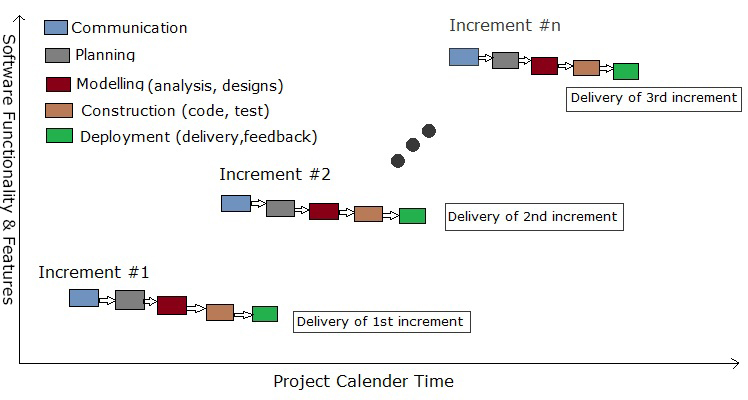
\includegraphics[width=0.7\linewidth]{Incremental-Development}
	\caption[Incremental Development]{\textcolor(blue){\url{http://www.robabdul.com/softwaredevelopment/software-development-cycle-for-data-management-system/}}}
	\label{fig:incremental-development}
\end{figure}

Successivamente ad un approfondita fase di analisi ed aver reso modulare ogni azione (\textit{BackLog}) cerchiamo comunque di eseguire i compiti possibili il più parallelamente possibile e singolarmente utilizzando un \textit{modello agile} di tipo \textbf{Scrum}.\\
In cui il \textit{Project Manager} si prende in carico la responsabilità di dare priorità ad ogni micro-obbiettivo che si deve eseguire e il team procede con la scrematura del lavoro . \\
La revisione in questi casi è giornaliera grazie al programma di messaggistica istantanea. Dove ogni mattina e ogni sera viene fatto un rendiconto rispettivamente del lavoro da svolgere e da quello che si è svolto.\\
Ogni compito è poi suddiviso in Asana così da essere chiaramente consultabile da ogni membro. Vi è flessibilità nella scelta, ogni componente può decidere a sua preferenza ciò da iniziare. Importante è essere sicuri di finire ciò che si è iniziato e il Project Manager ha la responsabilità di incaricare un membro nel caso di indugio.


\rhead{Pianificazione di Progetto}
\section{Pianificazione di Progetto}
Il gruppo SWEg ha deciso di suddividere lo sviluppo del progetto in cinque macro-fasi:
\begin{enumerate}
	\item \textbf{Analisi} (AN);
	\item \textbf{Analisi Dettaglio} (AD);
	\item \textbf{Progettazione Architetturale} (PA);
	\item \textbf{Progettazione di Dettaglio e Codifica} (PDC);
	\item \textbf{Validazione e Collaudo} (VC);
\end{enumerate}
Ogni macro-fase è poi stata suddivisa in attività più piccole, alle quali sono state associate una o più risorse. \\
Per facilità di scomposizione si è scelta una semplice divisione:
\begin{itemize}
	\item \textbf{Per capitoli}: ogni documento presenta dei capitoli prestabiliti e quindi un singolo può completare uno o più capitoli del documento.
	\item \textbf{Per azione}: a seconda di cui il singolo è specializzato ricopre un'attività inerente al suo ruolo. (Es: Esperto di produce un template, ecc...);
	\item \textbf{Verifica}: ogni documento e azione ha bisogno di verifica obbligatoria. Quindi è assegnata ai componenti in cui non vi è conflitto di interesse sulla stesura da parte del \textit{Project Manager}.
\end{itemize} 
La scomposizione non è segnata negli schemi. 
	

\subsection{Analisi}
\textit{\begin{center} Periodo: dal 04-11-2016 al 21-12-2016. \end{center}} 
Questo stadio inizia con la presentazione dei capitolati d'appalto e termina con la scadenza di
consegna della documentazione.
\\
Le attività nel punto di Analisi sono:
\begin{enumerate}
	\item \textbf{Studio di Fattibilità}: vengono valutati tutti i capitolati d'appalto e viene redatto uno studio di fattibilità.
	Viene studiata la complessità delle varie proposte mediante un abbozzo di \textit{Analisi dei Requisiti} ad alto livello.
	La prima attività da eseguire in quanto bloccante per l'\textit{Analisi dei Requisiti}. Concluso lo 
	studio di fattibilità si decide quale progetto il gruppo ambisce a realizzare;
	\item \textbf{Norme di progetto}: l'\textit{Amministratore} emana le norme che il gruppo sarà obbligato a seguire
	durante le attività. Sarà poi compito dei verificatori accertare il rispetto di tali norme;
	\item \textbf{Analisi dei Requisiti}: viene fatta un'analisi approfondita partendo dalla base fatta durante lo Studio di Fattibilità. Questa attività continuerà fino alla data di consegna;
	\item \textbf{Piano di Progetto}: il responsabile del gruppo redige questo documento così da organizzare le attività del gruppo. Questa attività ha un'alta priorità;
	\item \textbf{Piano di Qualifica}: l'\textit{Analista} redige il Piano di Qualifica in collaborazione con l'\textit{Amministratore} ed il \textit{Responsabile di Progetto}; 
	\item \textbf{Glossario}: viene scritto in modo incrementale da chi redige i documenti. Contiene la spiegazione di alcuni termini utilizzati. Viene redatto in parallelo a tutti i documenti ed è aggiornato ad ogni termine che necessita di una spiegazione;
	\item \textbf{Lettera di presentazione}: documento presentato al committente che permette al gruppo di partecipare alla gara d'appalto per il capitolato.
\end{enumerate}
In questa macro-fase i ruoli maggiormente coinvolti sono: \textit{Responsabile}, \textit{Amministratore}, \textit{Analista}. \\
Per facilità di rappresentazione lo schema è riportato insieme all' \textit{Analisi in Dettaglio}.

\subsection{Analisi in dettaglio}
\textit{\begin{center} Periodo: dal 22-12-2016 al 11-01-2017 \end{center}}
Questa sezione di progetto inizia dopo la \textit{Revisione dei Requisiti} e termina con l'inizio dell'attività di \textit{Progettazione Architetturale}.
In questa attività sostanzialmente viene migliorata l'\textit{Analisi dei Requisiti}.
\\
I ruoli maggiormente coinvolti sono il \textit{Responsabile}, l'\textit{Amministratore} e l'\textit{Analista}. \\

\begin{figure}
	\centering
	\includegraphics[width=1\linewidth]{"Gantt Analisi"}
	\caption{Analisi e Analisi in Dettaglio}
	\label{fig:gantt-progettazione-architetturale}
\end{figure}

\subsection{Progettazione Architetturale}
\begin{center}\textit{Periodo: dal 12-01-2017 al 27-02-2017}\end{center}
Questo punto termina con la consegna del prodotto
alla \textit{Revisione di Progetto}, lasciando l'attività successiva lo stato definitivo del prodotto stesso. Le attività in questo caso sono:
\begin{enumerate}
	\item \textbf{Specifica Tecnica}: il \textit{Progettista} espone le scelte progettuali che il prodotto dovrà avere.\\
	Verranno descritti i design pattern utilizzati nella creazione del prodotto, l'architettura generale del software, i principali flussi di controllo ed il tracciamento dei requisiti;
	\item \textbf{Incremento e verifica}: tutti i documenti verranno aggiornati in base al risultato della Revisione dei Requisiti.
\end{enumerate}
Le figure maggiormente coinvolte sono il \textit{Responsabile}, l'\textit{Amministratore}, il \textit{Progettista}, l'\textit{Analista}
ed il \textit{Verificatore}. \\

\begin{figure}
	\centering
	\includegraphics[width=1\linewidth]{"Gantt Progettazione Architetturale"}
	\caption{Progettazione Architetturale}
	\label{fig:gantt-progettazione-architetturale}
\end{figure}

\subsection{Progettazione di Dettaglio e Codifica}
\textit{\begin{center} Periodo: dal 28-02-2017 al 17-04-2015 \end{center}}
Inizia dopo la \textit{Revisione di Progetto} e termina con la consegna del prodotto alla \textit{Revisione di Qualifica}.\\
Le attività di questo stadio sono:
\begin{itemize}
	\item \textbf{Definizione di Prodotto}: viene definita la struttura in modo approfondito e le varie relazioni dei vari componenti del prodotto, basandosi sul documento di
\textit{Specifica Tecnica};
	\item \textbf{Codifica}: in questa fase inizia lo sviluppo del codice da parte dei programmatori, che devono seguire quanto riportato nel documento \textit{Definizione di Prodotto};
	\item \textbf{Manuale utente}: questo documento ha lo scopo di fornire delle linee guida per l'utilizzo del sistema;
	\item \textbf{Incremento e Verifica}: tutti i documenti verranno aggiornati in base al risultato della \textit{Revisione di Progettazione}.
\end{itemize}
I ruoli coinvolti sono il \textit{Responsabile}, l'\textit{Amministratore}, il \textit{Progettista}, il \textit{Verificatore}
ed il \textit{Programmatore}.\\

\begin{figure}
	\centering
	\includegraphics[width=1\linewidth]{"Gantt Progettazione di Dettaglio"}
	\caption{Progettazione di Dettaglio e Codifica}
	\label{fig:gantt-progettazione-di-dettaglio}
\end{figure}


\subsection{Validazione e Collaudo}
\textit{\begin{center} Periodo: dal 18-04-2017 al 14-05-2015 \end{center}}
Questa macro-sequenza riunisce tutti i test dalla più piccola quantità di software che conviene testare da sola al progetto complessivamente.\\
Ogni esame è correlato di un \textit{Analisi Statica} e \textit{Analisi Dinamica} che coincidono in modo complementare con una fase di progettazione e/o realizzazione.\\
Vi è l'obbligo di utilizzo di metodi automatici per la realizzazione dei test, onde evitare errori umani . Se nel corso del progetto si è svolta una verifica passo per passo, la validazione è spontanea. \\ 
Rappresenta l'atto conclusivo delle varie attività di verifica realizzate nei singoli processi del ciclo di vita.
Le attività sono:
\begin{enumerate}
	\item \textbf{Test di Unità};
	\item \textbf{Test di Integrazione};
	\item \textbf{Test di Sistema};
	\item \textbf{Collaudo};
	\item \textbf{Validazione}: controllo generico di tutti i documenti.
\end{enumerate}
I ruoli coinvolti sono il \textit{Responsabile}, l'\textit{Amministratore}, il \textit{Progettista} ed il \textit{Verificatore}.

\begin{figure}
	\centering
	\includegraphics[width=1\linewidth]{"Gantt Validazione e Collaudo"}
	\caption{Validazione e Collaudo}
	\label{fig:gantt-validazione-e-collaudo}
\end{figure}


\newpage

\rhead{Preventivo}
\section{Preventivo}
Qui vengono presentati, per ogni fase del progetto, le ore preventivate di impiego per i vari ruoli coinvolti.\\
Si ricorda che le fasi di \textit{Analisi dei Requisiti} e \textit{Analisi Dettaglio} non sono a carico del committente e quindi non saranno considerate nel calcolo delle ore totali da retribuire. \\
Costi e sigle delle tabelle fanno riferimento al capitolo \textit{Ruoli} del documento: \textit{Norme di Progetto}.

\subsection{Analisi}
Nella fase di analisi non vi sono ore di \textit{Codifica}, eseguite dal \textit{Programmatore}, e di \textit{Progettazione}, eseguite dal \textit{Progettista}. Questo perché Analisi e Progettazione non sono mai simultaneamente attive. \\
Durante il periodo di Analisi le ore tra i ruoli sono state divise nel modo seguente: \\

{\renewcommand\arraystretch{1.2} %aumenta l'altezza di ogni riga
\begin{tabular}{|c|c|c|c|c|c|c|c|}
	\hline 
	\textbf{Nome} & \multicolumn{6}{c|}{\textbf{Ore e Costo per Ruolo}} & \textbf{Costo totale} \\ 
	& \textbf{PM} & \textbf{AM} & \textbf{AN} & \textbf{PL} & \textbf{PR} & \textbf{VE} & \textbf{ \euro } \\ 
	\hline
	Sebastiano Marchesini & 8x30 & 9x20 & 4x25 & & & & 520,00 \\ 
	\hline 
	Gianluca Crivellaro & & & 18x25 & & & 3x15 & 495,00 \\ 
	\hline 
	Pietro Lonardi & & & 13x25 & & & 7x15 & 430,00 \\ 
	\hline 
	Alberto Gelmi & & & 8x25 & & & 7x15 & 305,00 \\ 
	\hline 
	Piergiorgio Danieli & 5x30 & 5x20 & & & & 12x15 & 430,00 \\ 
	\hline 
	\multicolumn{7}{r|}{TOTALE :} & \textit{\euro 2180,00} \\ 
\end{tabular}} 

\subsection{Analisi Dettaglio}
Analisi Dettaglio concentra tutto il team sul documento di \textit{Analisi dei Requisiti}. Ognuno pone la sua attenzione su un particolare argomento del progetto, si analizza, guidati dal \textit{Project Manager}. L'\textit{Amministratore} è a capo delle revisioni . Non vi sono altri compiti da svolgere in questo stadio, quindi non vi sono altre ore rendicontate.\\
Nel periodo che riguarda l'Analisi Dettaglio, le ore tra i ruoli sono state divise come segue:\\

{\renewcommand\arraystretch{1.2} %aumenta l'altezza di ogni riga
	\begin{tabular}{|c|c|c|c|c|c|c|c|}
		\hline 
		\textbf{Nome} & \multicolumn{6}{c|}{\textbf{Ore e Costo per Ruolo}} & \textbf{Costo totale} \\ 
		& \textbf{PM} & \textbf{AM} & \textbf{AN} & \textbf{PL} & \textbf{PR} & \textbf{VE} & \textbf{ \euro } \\ 
		\hline
		Sebastiano Marchesini & & & 1x25 & & & 3x15 & 70,00 \\ 
		\hline 
		Gianluca Crivellaro & 1x30 & & 4x25 & & & 1x15 & 145,00 \\ 
		\hline 
		Pietro Lonardi & & 1x20 & 3x25 & & & 2x15 & 125,00 \\ 
		\hline 
		Alberto Gelmi & & & 3x25 & & & 1x15 & 90,00 \\ 
		\hline 
		Piergiorgio Danieli & & & 2x25 & & & 3x15 & 95,00 \\ 
		\hline 
		\multicolumn{7}{r|}{TOTALE :} & \textit{\euro 525,00} \\ 
\end{tabular}} 

\subsection{Progettazione Architetturale}
Anche in questa fase viene meno un ruolo del team che può svolgere solo una funzione: quella del \textit{Programmatore}. Trovare soluzioni alle analisi rilevate non è suo compito ma solo di tradurre in linguaggio di programmazione le decisione del \textit{Progettista}.
Nel periodo riguardante la fase di Progettazione Architetturale le ore tra i ruoli sono stati divisi nel seguente modo:\\

{\renewcommand\arraystretch{1.2} %aumenta l'altezza di ogni riga
	\begin{tabular}{|c|c|c|c|c|c|c|c|}
		\hline 
		\textbf{Nome} & \multicolumn{6}{c|}{\textbf{Ore e Costo per Ruolo}} & \textbf{Costo totale} \\ 
		& \textbf{PM} & \textbf{AM} & \textbf{AN} & \textbf{PL} & \textbf{PR} & \textbf{VE} & \textbf{ } \\ 
		\hline 
		Sebastiano Marchesini & & & 5x25 & 13x22 & & 7x15 & 516,00 \\ 
		\hline 
		Gianluca Crivellaro & 3x30 & & 2x25 & 14x22 & & 4x15 & 508,00 \\ 
		\hline 
		Pietro Lonardi & & 2x20 & 2x25 & 11x22 & & 9x15 & 467,00 \\ 
		\hline 
		Alberto Gelmi & 3x30 & & 4x25 & 18x22 & & 3x15 & 631,00 \\ 
		\hline 
		Piergiorgio Danieli & & & 2x25 & 14x22 & & 7x15 & 463,00 \\ 
		\hline 
		\multicolumn{7}{r|}{TOTALE :} & \textit{\euro 2594,00} \\ 
\end{tabular}} 

\subsection{Progettazione di Dettaglio e Codifica}
Oramai tutta l'analisi è completata e quindi il ruolo dell'\textit{Analista} è praticamente sostituito dal \textit{Progettista}. Inoltre la codifica apre le porte alla programmazione effettiva e quindi al ruolo di \textit{Programmatore}.\\
Durante la fase di Progettazione di Dettaglio e Codifica le ore tra i ruoli sono stai divisi come segue:
\\

{\renewcommand\arraystretch{1.2} %aumenta l'altezza di ogni riga
	\begin{tabular}{|c|c|c|c|c|c|c|c|}
		\hline 
		\textbf{Nome} & \multicolumn{6}{c|}{\textbf{Ore e Costo per Ruolo}} & \textbf{Costo totale} \\ 
		& \textbf{PM} & \textbf{AM} & \textbf{AN} & \textbf{PL} & \textbf{PR} & \textbf{VE} & \textbf{ \euro } \\ 
		\hline
		Sebastiano Marchesini & & & & 22x22 & 29x15 & & 919,00 \\ 
		\hline 
		Gianluca Crivellaro & & 3x20 & & 18x22 & 19x15 & 2x15 & 815,00 \\ 
		\hline 
		Pietro Lonardi & 3x30 & & & 19x22 & 3x15 & 25x15 & 847,00 \\ 
		\hline 
		Alberto Gelmi & 5x30 & & 2x25 & 4x22 & 28x15 & 11x15 & 873,00 \\ 
		\hline 
		Piergiorgio Danieli & & & & 20x22 & 27x15 & & 845,00 \\ 
		\hline 
		\multicolumn{7}{r|}{TOTALE :} & \textit{\euro 4299,00} \\ 
\end{tabular}} 

\subsection{Validazione e Collaudo}
Nella fase di Validazione e Collaudo le ore tra i ruoli sono state divise nel seguente modo:
\\

{\renewcommand\arraystretch{1.2} %aumenta l'altezza di ogni riga
	\begin{tabular}{|c|c|c|c|c|c|c|c|}
		\hline 
		\textbf{Nome} & \multicolumn{6}{c|}{\textbf{Ore e Costo per Ruolo}} & \textbf{Costo totale} \\ 
		& \textbf{PM} & \textbf{AM} & \textbf{AN} & \textbf{PL} & \textbf{PR} & \textbf{VE} & \textbf{ \euro } \\ 
		\hline
		Sebastiano Marchesini & 2x30 & & & & 1x15 & 1x15 & 90 \\ 
		\hline 
		Gianluca Crivellaro & & 1x20 & & & & 2x15 & 50 \\ 
		\hline 
		Pietro Lonardi & & & & 1x22 & 2x15 & 2x15 & 82 \\ 
		\hline 
		Alberto Gelmi & & 2x20 & & 2x22 & 2x15 & 2x15 & 144 \\ 
		\hline 
		Piergiorgio Danieli & 1x30 & & & & 2x15 & 3x15 & 105 \\ 
		\hline 
		\multicolumn{7}{r|}{TOTALE :} & \textit{\euro 471,00} \\ 
\end{tabular}} 

\subsection{Riepilogo}
Le ore totali previste per la realizzazione dell'intero progetto, comprese le ore di investimento, sono le seguenti: \\

{\renewcommand\arraystretch{1.2} %aumenta l'altezza di ogni riga
	\begin{tabular}{|c|c|c|c|c|c|c|c|}
			\hline 
		\textbf{Nome} & \multicolumn{6}{c|}{\textbf{Ore per Ruolo Totali}} & \textbf{Ore Totali} \\ 
		& \textbf{PM} & \textbf{AM} & \textbf{AN} & \textbf{PL} & \textbf{PR} & \textbf{VE} & \\ 
		\hline
		Sebastiano Marchesini	& 10 & 9 & 10 & 35 & 30 & 11 & 105 \\ 
		\hline 
		Gianluca Crivellaro 	& 4 & 4 & 34 & 30 & 21 & 12 & 105 \\ 
		\hline 
		Pietro Lonardi 			& 3 & 3 & 18 & 31 & 5 & 45 & 105 \\ 
		\hline 
		Alberto Gelmi 			& 8 & 2 & 19 & 24 & 30 & 25 & 105 \\ 
		\hline 
		Piergiorgio Danieli 	& 6 & 5 & 4 & 36 & 29 & 25 & 105 \\ 
		\hline 
		\multicolumn{7}{r|}{TOTALE :} & 525 \\ 
\end{tabular}} 


\newpage

\rhead{Consuntivo di Periodo}
\section{Consuntivo di Periodo}
Riepiloga i risultati di un dato periodo di attività e verrà aggiornato nel corso del progetto per dare una rendiconto preciso ed effettivo del lavoro svolto. \\
\subsection{Analisi e Analisi Dettaglio}

{\renewcommand\arraystretch{1.2}  %aumenta l'altezza di ogni riga
	\begin{tabular}{|c|c|c|c|c|c|c|c|}
		\hline 
		\textbf{Nome} & \multicolumn{6}{c|}{\textbf{Ore Effettive per Ruolo}} & \textbf{Ore Totali} \\ 
		& \textbf{PM} & \textbf{AM} & \textbf{AN} & \textbf{PL} & \textbf{PR} & \textbf{VE} & \\ 
		\hline
		Sebastiano Marchesini & 8 & 10(+1) & 5 &  &  & 4(+1) & 27(+2) \\ 
		\hline 
		Gianluca Crivellaro & 1 &  & 24(+2) &  &  & 3 & 28(+2) \\ 
		\hline 
		Pietro Lonardi &  & 1 & 6 &  &  & 9(+2) & 17(+2) \\ 
		\hline 
		Alberto Gelmi &  &  & 9(-2) &  &  & 8 & 17(-2) \\ 
		\hline 
		Piergiorgio Danieli & 5 & 5 & 2 &  &  & 5 & 17(+0) \\ 
		\hline 
		\multicolumn{7}{r|}{TOTALE  :} & 106(+4) \\ 
\end{tabular}} 


\newpage

\rhead{Preventivo a Finire}
\section{Preventivo a Finire}
Il preventivo finale va a sommare tutte i costi ad ora organizzati. Si tiene conto del massimo impegno e della qualità scelta negli standard proposti. \\
Non vengono tenute in considerazione:
\begin{itemize}
	\item manutenzione e preparazione dell'hardware,
	\item attività di auto-formazione per quanto concerne la strumentazione e le specifiche.
	\item le ore di \textit{Analisi} e \textit{Analisi in Dettaglio}
\end{itemize}

\subsection{Preventivo Finale}
{\renewcommand\arraystretch{1.2} %aumenta l'altezza di ogni riga
\begin{tabular}{|c|c|c|}
	\hline 
	& \textbf{Costo} & \textbf{Costo Effettivo} \\ 
	\hline 
	\textbf{Analisi} & 2180,00 & 00,00 \\ 
	\hline 
	\textbf{Analisi Specifica} & 525,00 & 00,00 \\ 
	\hline 
	\textbf{Progettazione} & 2594,00 & 2594,00 \\ 
	\hline 
	\textbf{Progettazione in Dettaglio e Codifica} & 4299,00 & 4299,00 \\ 
	\hline 
	\textbf{Validazine e Collaudo} & 471,00 & 471,00 \\ 
	\hline 
	\multicolumn{2}{r|}{TOTALE :} & \textit{\euro 7334,00 } \\ 
\end{tabular}
} 
\vspace{0.5cm}

In seguito riporteremo i danni economici che vi sono riportati confrontando il preventivo con l'effettivo consuntivo di periodo.

\end{document}